\section{Web Service API}\label{design:web_service}
The web service API was implemented using ASP.NET Web API 2.3\cite{aspnet_webapi}.
ASP.NET Web API uses ASP.NET MVC\cite{aspnet_mvc}, with the use of \texttt{ApiController}, instead of the regular \texttt{Controller}.
In the architecture, the web service is defined as a component of its own (see \Cref{arch:webservice}).
\mikkel{Jeg sidder tilbage med en følelse af ''øhh'' når jeg læser det her.}

\subsection{Resource Oriented Architecture}
Resource Oriented Architecture criteria, as described in \Cref{webservice:roa}, set the ground rules for designing the API.
These criteria are therefore upheld by the API.
\mikkel{Er det nødvendigt med en ROA subsection. Kan vi ikke bare nævne det som en paragraph og lave Resources om til en subsection?}

\subsubsection{Resources}\label{webservice:resources}
This section contains the resources designed and implemented in the web service.
Resources in the implementation are objects, containing named properties and sub-resources.
Sub-resources are represented as simple objects, containing only its relative URL.
Each resource is described following this structure:
\begin{itemize}
\item \textbf{URL} the URL of the resource
\item \textbf{Properties} a property which can be accessed from this resource
\item \textbf{Resources} the resource(s) which can be accessed from this resource
\item \textbf{Methods} HTTP methods which can be used on that resource
\item \textbf{Responses} HTTP status codes which could be returned by this resource
\end{itemize}

\subsubsection*{The resources implemented:}
% Command for displaying url, properties, and sub-resource of each resource
\newcommand{\resource}[6]{\noindent \vfill \fbox{\begin{minipage}{\textwidth}\begin{description}
\item[URL:]{\texttt{#1}}
\item[Properties:]{\texttt{#2}}
\item[Resources:]{\texttt{#3}}
\item[Methods:]{\texttt{#4}}
\item[Responses:]{\texttt{#5}}
\end{description}
{#6}
\end{minipage}
}\vfill }

\resource{/}{version}{availablebikes, hotspots, predictions}{GET}{200 OK}
{The root path serves as the entry point for the API.
It has a single property; version, to be used for asserting that the API has changes that implementations should react to.
More importantly, it contains a sub-resource for each main resource.}

\resource{/availablebikes}{count}{List of availablebikes}{GET}{200 OK}
{This resource contains a list of all \texttt{availablebike} resources, along with a count of how many there are.}


\resource{/availablebikes/\{bikeId\}}{latitude, longitude}{}{GET}{200 OK, 404 Not Found}
{This is the actual \texttt{availablebike} resource.
In case a client tries to request a bike that is not available, it will be met with a \texttt{404 Not Found} response.}


\resource{/hotspots}{hotspots}{}{GET}{200 OK}
{This resource returns all the hotspots in the system.}



\resource{/predictions}{}{}{GET}{200 OK}
{This is the prediction resource.
When a client wants to know when a bike arrives at a hotspot this resource can be used.}
\mikkel{Jeg tænker at vi kan gøre repræsentationen af vores resourcer enklere.}

\subsection{MVC} 
MVC or Model-View-Controller\cite{aspmvc} is used to separate responsibility of an application into three parts, the model, the view, and the controller.
The pattern can be seen in \Cref{mvcdiagram}.

\begin{figure}[h]
\begin{center}
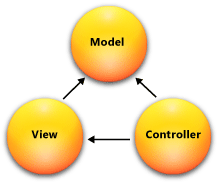
\includegraphics[width=\textwidth, trim={-4cm 11cm 5cm 1cm}]{mvc.pdf}
\caption{The MVC design pattern.}
\label{mvcdiagram}
\end{center}
\end{figure}

\paragraph{Model} contains the model of the application domain and takes care of fetching data and making it available through the model.

In the case of our web service, the model is making resources available for the view.

\paragraph{View} displays the model to the user.
In our case the view is the serialized resource representation, that the user obtains by performing requests against the API.
Per default, this is \texttt{text/xml}, however, by adding the \texttt{Accept} header, this can be set to \texttt{application/json} \cite[Section 14]{http_specification}.

\paragraph{Controller} handles the interaction with users.
Based on user input, the controller works on the model and selects what the view needs to be used for displaying the data.

The routing to controllers is handled by the attributes \texttt{[RoutePrefix]} and \texttt{[Route]}.
In order to handle the different HTTP methods, controller methods are also annotated with an appropriate \texttt{[Http\{Method\}]} attribute (e.g. \texttt{[HttpGet]}) \cite{asp_routing}.

